% Options for packages loaded elsewhere
\PassOptionsToPackage{unicode}{hyperref}
\PassOptionsToPackage{hyphens}{url}
%
\documentclass[
]{article}
\usepackage{lmodern}
\usepackage{amssymb,amsmath}
\usepackage{ifxetex,ifluatex}
\ifnum 0\ifxetex 1\fi\ifluatex 1\fi=0 % if pdftex
  \usepackage[T1]{fontenc}
  \usepackage[utf8]{inputenc}
  \usepackage{textcomp} % provide euro and other symbols
\else % if luatex or xetex
  \usepackage{unicode-math}
  \defaultfontfeatures{Scale=MatchLowercase}
  \defaultfontfeatures[\rmfamily]{Ligatures=TeX,Scale=1}
\fi
% Use upquote if available, for straight quotes in verbatim environments
\IfFileExists{upquote.sty}{\usepackage{upquote}}{}
\IfFileExists{microtype.sty}{% use microtype if available
  \usepackage[]{microtype}
  \UseMicrotypeSet[protrusion]{basicmath} % disable protrusion for tt fonts
}{}
\makeatletter
\@ifundefined{KOMAClassName}{% if non-KOMA class
  \IfFileExists{parskip.sty}{%
    \usepackage{parskip}
  }{% else
    \setlength{\parindent}{0pt}
    \setlength{\parskip}{6pt plus 2pt minus 1pt}}
}{% if KOMA class
  \KOMAoptions{parskip=half}}
\makeatother
\usepackage{xcolor}
\IfFileExists{xurl.sty}{\usepackage{xurl}}{} % add URL line breaks if available
\IfFileExists{bookmark.sty}{\usepackage{bookmark}}{\usepackage{hyperref}}
\hypersetup{
  pdftitle={The Influence of Individual Characterisitcs on Public Transportation Planning},
  pdfauthor={Iris Zhong},
  hidelinks,
  pdfcreator={LaTeX via pandoc}}
\urlstyle{same} % disable monospaced font for URLs
\usepackage[margin=1in]{geometry}
\usepackage{color}
\usepackage{fancyvrb}
\newcommand{\VerbBar}{|}
\newcommand{\VERB}{\Verb[commandchars=\\\{\}]}
\DefineVerbatimEnvironment{Highlighting}{Verbatim}{commandchars=\\\{\}}
% Add ',fontsize=\small' for more characters per line
\usepackage{framed}
\definecolor{shadecolor}{RGB}{248,248,248}
\newenvironment{Shaded}{\begin{snugshade}}{\end{snugshade}}
\newcommand{\AlertTok}[1]{\textcolor[rgb]{0.94,0.16,0.16}{#1}}
\newcommand{\AnnotationTok}[1]{\textcolor[rgb]{0.56,0.35,0.01}{\textbf{\textit{#1}}}}
\newcommand{\AttributeTok}[1]{\textcolor[rgb]{0.77,0.63,0.00}{#1}}
\newcommand{\BaseNTok}[1]{\textcolor[rgb]{0.00,0.00,0.81}{#1}}
\newcommand{\BuiltInTok}[1]{#1}
\newcommand{\CharTok}[1]{\textcolor[rgb]{0.31,0.60,0.02}{#1}}
\newcommand{\CommentTok}[1]{\textcolor[rgb]{0.56,0.35,0.01}{\textit{#1}}}
\newcommand{\CommentVarTok}[1]{\textcolor[rgb]{0.56,0.35,0.01}{\textbf{\textit{#1}}}}
\newcommand{\ConstantTok}[1]{\textcolor[rgb]{0.00,0.00,0.00}{#1}}
\newcommand{\ControlFlowTok}[1]{\textcolor[rgb]{0.13,0.29,0.53}{\textbf{#1}}}
\newcommand{\DataTypeTok}[1]{\textcolor[rgb]{0.13,0.29,0.53}{#1}}
\newcommand{\DecValTok}[1]{\textcolor[rgb]{0.00,0.00,0.81}{#1}}
\newcommand{\DocumentationTok}[1]{\textcolor[rgb]{0.56,0.35,0.01}{\textbf{\textit{#1}}}}
\newcommand{\ErrorTok}[1]{\textcolor[rgb]{0.64,0.00,0.00}{\textbf{#1}}}
\newcommand{\ExtensionTok}[1]{#1}
\newcommand{\FloatTok}[1]{\textcolor[rgb]{0.00,0.00,0.81}{#1}}
\newcommand{\FunctionTok}[1]{\textcolor[rgb]{0.00,0.00,0.00}{#1}}
\newcommand{\ImportTok}[1]{#1}
\newcommand{\InformationTok}[1]{\textcolor[rgb]{0.56,0.35,0.01}{\textbf{\textit{#1}}}}
\newcommand{\KeywordTok}[1]{\textcolor[rgb]{0.13,0.29,0.53}{\textbf{#1}}}
\newcommand{\NormalTok}[1]{#1}
\newcommand{\OperatorTok}[1]{\textcolor[rgb]{0.81,0.36,0.00}{\textbf{#1}}}
\newcommand{\OtherTok}[1]{\textcolor[rgb]{0.56,0.35,0.01}{#1}}
\newcommand{\PreprocessorTok}[1]{\textcolor[rgb]{0.56,0.35,0.01}{\textit{#1}}}
\newcommand{\RegionMarkerTok}[1]{#1}
\newcommand{\SpecialCharTok}[1]{\textcolor[rgb]{0.00,0.00,0.00}{#1}}
\newcommand{\SpecialStringTok}[1]{\textcolor[rgb]{0.31,0.60,0.02}{#1}}
\newcommand{\StringTok}[1]{\textcolor[rgb]{0.31,0.60,0.02}{#1}}
\newcommand{\VariableTok}[1]{\textcolor[rgb]{0.00,0.00,0.00}{#1}}
\newcommand{\VerbatimStringTok}[1]{\textcolor[rgb]{0.31,0.60,0.02}{#1}}
\newcommand{\WarningTok}[1]{\textcolor[rgb]{0.56,0.35,0.01}{\textbf{\textit{#1}}}}
\usepackage{graphicx,grffile}
\makeatletter
\def\maxwidth{\ifdim\Gin@nat@width>\linewidth\linewidth\else\Gin@nat@width\fi}
\def\maxheight{\ifdim\Gin@nat@height>\textheight\textheight\else\Gin@nat@height\fi}
\makeatother
% Scale images if necessary, so that they will not overflow the page
% margins by default, and it is still possible to overwrite the defaults
% using explicit options in \includegraphics[width, height, ...]{}
\setkeys{Gin}{width=\maxwidth,height=\maxheight,keepaspectratio}
% Set default figure placement to htbp
\makeatletter
\def\fps@figure{htbp}
\makeatother
\setlength{\emergencystretch}{3em} % prevent overfull lines
\providecommand{\tightlist}{%
  \setlength{\itemsep}{0pt}\setlength{\parskip}{0pt}}
\setcounter{secnumdepth}{5}
\usepackage{booktabs}
\usepackage{setspace}
\doublespacing
\usepackage[labelfont=bf]{caption}
\usepackage{booktabs}
\usepackage{longtable}
\usepackage{array}
\usepackage{multirow}
\usepackage{wrapfig}
\usepackage{float}
\usepackage{colortbl}
\usepackage{pdflscape}
\usepackage{tabu}
\usepackage{threeparttable}
\usepackage{threeparttablex}
\usepackage[normalem]{ulem}
\usepackage{makecell}
\usepackage{xcolor}

\title{The Influence of Individual Characterisitcs on Public Transportation
Planning\thanks{xx}}
\author{Iris Zhong}
\date{}

\begin{document}
\maketitle
\begin{abstract}
xx
\end{abstract}

\begin{verbatim}
## Warning: package 'tidyverse' was built under R version 3.5.3
\end{verbatim}

\begin{verbatim}
## Warning: package 'ggplot2' was built under R version 3.5.3
\end{verbatim}

\begin{verbatim}
## Warning: package 'tibble' was built under R version 3.5.3
\end{verbatim}

\begin{verbatim}
## Warning: package 'tidyr' was built under R version 3.5.3
\end{verbatim}

\begin{verbatim}
## Warning: package 'readr' was built under R version 3.5.3
\end{verbatim}

\begin{verbatim}
## Warning: package 'purrr' was built under R version 3.5.3
\end{verbatim}

\begin{verbatim}
## Warning: package 'dplyr' was built under R version 3.5.3
\end{verbatim}

\begin{verbatim}
## Warning: package 'stringr' was built under R version 3.5.3
\end{verbatim}

\begin{verbatim}
## Warning: package 'forcats' was built under R version 3.5.3
\end{verbatim}

\begin{verbatim}
## Warning: package 'lubridate' was built under R version 3.5.3
\end{verbatim}

\begin{verbatim}
## Warning: package 'stargazer' was built under R version 3.5.2
\end{verbatim}

\begin{verbatim}
## Warning: package 'corrplot' was built under R version 3.5.3
\end{verbatim}

\begin{verbatim}
## Warning: package 'Hmisc' was built under R version 3.5.3
\end{verbatim}

\begin{verbatim}
## Warning: package 'survival' was built under R version 3.5.3
\end{verbatim}

\begin{verbatim}
## Warning: package 'Formula' was built under R version 3.5.2
\end{verbatim}

\begin{verbatim}
## Warning: package 'dlookr' was built under R version 3.5.3
\end{verbatim}

\begin{verbatim}
## Warning: package 'mice' was built under R version 3.5.3
\end{verbatim}

\begin{verbatim}
## Warning: package 'car' was built under R version 3.5.3
\end{verbatim}

\begin{verbatim}
## Warning: package 'carData' was built under R version 3.5.3
\end{verbatim}

\begin{verbatim}
## Warning: package 'patchwork' was built under R version 3.5.3
\end{verbatim}

\hypertarget{literature-review}{%
\section{Literature Review}\label{literature-review}}

Allen et al.~(2016) study the reasoning of the failure of a referendum
on a congestion charging scheme in Edinburgh. Instead of using direct
voting data, they conduct a survey after the referendum, which allows
them to ask more specific questions. Researchers can gain detailed data
by surveying, because the unit of measurement is each individual;
however, a possible disadvantage of surveying is that respondents who
turn in the questionnaire tend to have stronger attitudes towards the
proposal, generating sampling bias. They conclude that people who use
cars as the primary transportation mean, demonstrate a misconception of
the pricing plan, or question the effectiveness of the scheme at
reducing congestion are more likely to oppose it. Their findings can
give insights to the similar failure in the Gwinnett referendum. Voters
against the proposal could be those who rarely use public transportation
and those who are not convinced by the effectiveness of expanding public
transit in alleviating the traffic.

Another crucial factor is the accessibility of the proposed transit
system. Kinsey et al.~(2010) examine the relationship between the
distance to the scheduled railway station and voter turnout by studying
the Seattle monorail referendum. They introduce the concept of diffused
and concentrated benefit/cost. People who live far from the monorail
enjoy the diffused benefit of less traffic congestion, and bear the
diffused cost of increased tax. People living close to the rail
experience the same diffused benefit and cost, but they also gain the
concentrated benefit of easily accessing the public good. Finally, those
who live very close to the railway have the same benefits and costs, but
they also face the concentrated cost such as inconvenience during
construction. Since ``people are more strongly motivated to avoid losses
than to approach gains,'' they expect a higher turnout rate in farther
places with votes for ``no,'' which is verified from their analyses.
Besides distance, they also find out precincts with a higher percentage
of people of lower socioeconomic status or young people have a lower
turnout rate. Interestingly, there is a significant interaction between
partisanship and distance, which would be also tested in my study. In
essence, the effect of distance on turnout is weakened by partisanship,
and vanishes beyond a threshold of distance. Even though my dependent
variable is voters' responses rather than turnout, it can be inferred
from Kinsey et al.'s findings that people farther away from the transit
system would vote against the referendum more. However, the relationship
might be non-linear and requires some form of transformation. Regarding
the methods, they utilize the spatial lag model to correct for
autocorrelation, which is proper to use in my project as well since both
studies use precinct-level data.

\hypertarget{background}{%
\section{Background}\label{background}}

\hypertarget{current-transportation}{%
\subsection{current transportation}\label{current-transportation}}

\hypertarget{connect-gwinnett-transit-plan}{%
\subsection{Connect Gwinnett: Transit
Plan}\label{connect-gwinnett-transit-plan}}

\hypertarget{plan-overview}{%
\subsubsection{Plan overview}\label{plan-overview}}

\hypertarget{financing}{%
\subsubsection{Financing}\label{financing}}

\hypertarget{referendum}{%
\subsection{referendum}\label{referendum}}

\hypertarget{data-methods}{%
\section{Data \& Methods}\label{data-methods}}

\hypertarget{conceptual-model}{%
\subsection{Conceptual model}\label{conceptual-model}}

According to previous research, sociodemographic elements can influence
people's voting decisions in the referendum. For example, the effect of
income is mixed: on the one hand, people with higher income will pay a
smaller portion of their earnings for the implementation of the plan; on
the other hand, they will pay a larger amount of tax. Bollino (2008)
finds a positive correlation between income and people's willingness to
pay for renewable resources. Burkhardt and Chan (2017) separate the
influence of income from tax, and discover their opposite effects on
voting. Therefore, it is worth considering the relationship between
income and percentage of supporters in this referendum. Voters'
partisanship attachment is found to be a significant factor as well in
Burkhardt and Chan's (2017) paper. Areas with higher proportions of
Republicans are less supportive of fiscally costly propositions. In my
project, it can be hypothesized that tracts that have a higher
proportion of Trump supporters tend to have a lower percentage of
agreement to the proposal.

In addition, some factors related to transportation can intuitively
shape people's attitudes towards public transit. For example, the areas
in which people do not use public transit at all might have a higher
percentage of refusal of the proposal. People who have to travel a long
time to work are more likely to support the extension plan if it helps
save time. These two factors serve as controls in the models.

Finally, people favor the proposition if it benefits them. Specifically,
tracts that are not covered by public transport at present but will be
covered in the expansion plan are predicted to support the proposal
more.

\hypertarget{data}{%
\subsection{Data}\label{data}}

The ballot results of the Gwinnett County referendum on Mar 19th, 2019
is obtained from a website powered by Scytl, a trusted source of
election outcomes. The cross-sectional dataset contains the voting
information of all 157 precincts in the county. The dependent variable
-- the proportion of supporters of the referendum, and the voter turnout
rate are calculated from this data source.

The result of the 2016 Presidential Election is chosen to reflect
partisanship. A cross-sectional precinct-level election data is obtained
from the MIT Election Data and Science Lab website. The number of votes
for Trump at each precinct in Gwinnett county comes from this dataset.

Next, cross-sectional sociodemographic characteristics at the census
tract level are found in Census Bureau via an R package called
\texttt{tidycensus}. The data comes from the American Community Survey
5-year estimate published in 2018. The median age and median income are
collected here. In addition, the proportion of white, the percentage of
people who go to work by public transportation, and the percentage of
people who travel more than an hour to work are calculated by dividing
the relevant variables by the total population or the survey sample
size.

The information on whether the tract enjoys the proximity of public
transportation now and future can be acquired from spatial maps and
analyses. First, a precinct-level shapefile of Gwinnett County made in
2018 is obtained from the Georgia General Assembly. Gwinnett County maps
with current and proposed future public transit systems are available on
the Gwinnett County government website. I select the short-range
expansion plan (Y2020 -- 2025) because the cost and benefit of the
expansion in the far future are discounted more. After modifications in
QGIS software, the maps are then transformed into spatial data readable
in R. Five-hundred-meter buffer zones are created around bus and railway
routes. The categorical variable \emph{current\_plan} has four levels: 1
represents no transportation near this tract at present and in the
future; 2 represents the tracts that are accessible to public transit
currently but not in the future; 3 stands for the tracts that do not
have transit at present but will do in the expansion plan; 4 represents
the tracts that have and will have public transit for now and for the
future.

As noted above, both referendum and 2016 election data are collected at
the precinct level. However, the other datasets are performed at the
census tract level. Therefore, referendum and election data are
redistributed by the areas shared by the precinct and the tract. See the
data appendix for detailed steps of transformation.

The final dataset joins the datasets above by GEOID. It is
cross-sectional, measured with the unit of the census tract. Since there
are 113 census tracts in Gwinnett, the dataset has 113 observations,
with no missing data. A description of the variables can be found in
\emph{Table 1}.

\begin{table}
\centering
\caption{Variable definitions}
\label{variableDefinitions}
\begin{tabular}{ll}
\hline
\hline
Variable name      & Description                                   \\
\hline
GEOID          & The geographic identifier of the census tract                 \\
medage        & The median age of the population in the tract               \\
medincome        & The median income of the population in the tract               \\
white\_pct           & The percentage of white population in the tract      \\
public\_pct          & The percentage of people who go to work by public transportation (excluding taxi or cab)      \\
time\_pct           & The percentage of people who travel more than an hour to work      \\
trump\_pct          & The estimated percentage of votes for Donald Trump in that tract      \\
voter\_turnout  & The estimated percentage of voters who voted in this referendum in the tract \\
yes\_pct           & The estimated percentage of voters who voted yes in this referendum in the tract      \\
plan\_yes          & Whether the tract is covered by the public transportation now and in the short-range, \\ & defined by whether any transportation is available within 500 meters. \\ & 1 stands for the tract doesn't have transit both now and in the short-range plan. \\ & 2 stands for the tract has transit now but not in the short-range plan. \\ & 3 stands for the tract that doesn't have transit now and will have in the future.\\ & 4 stands for the tract that has public transit both now and in the future      \\

\hline
\end{tabular}
\end{table}

\begin{table}[!htbp] \centering 
  \caption{Summary statistics} 
  \label{summaryStats} 
\begin{tabular}{@{\extracolsep{5pt}}lccccccc} 
\\[-1.8ex]\hline 
\hline \\[-1.8ex] 
Statistic & \multicolumn{1}{c}{N} & \multicolumn{1}{c}{Mean} & \multicolumn{1}{c}{St. Dev.} & \multicolumn{1}{c}{Min} & \multicolumn{1}{c}{Pctl(25)} & \multicolumn{1}{c}{Pctl(75)} & \multicolumn{1}{c}{Max} \\ 
\hline \\[-1.8ex] 
medage & 113 & 35.56 & 4.58 & 26 & 32.8 & 38.8 & 52 \\ 
medincome & 113 & 69,439.24 & 24,358.44 & 33,020 & 51,429 & 82,845 & 156,136 \\ 
white\_pct & 113 & 0.48 & 0.15 & 0.17 & 0.38 & 0.61 & 0.89 \\ 
public\_pct & 113 & 0.01 & 0.01 & 0 & 0.002 & 0.02 & 0 \\ 
time\_pct & 113 & 0.16 & 0.05 & 0.04 & 0.12 & 0.20 & 0.31 \\ 
trump\_pct & 113 & 0.40 & 0.15 & 0.11 & 0.27 & 0.52 & 0.69 \\ 
voter\_turnout & 113 & 0.16 & 0.06 & 0.05 & 0.13 & 0.18 & 0.37 \\ 
yes\_pct & 113 & 0.53 & 0.14 & 0.27 & 0.42 & 0.61 & 0.84 \\ 
\hline \\[-1.8ex] 
\end{tabular} 
\end{table}

\begin{Shaded}
\begin{Highlighting}[]
\NormalTok{data_numeric <-}\StringTok{ }\NormalTok{final_data }\OperatorTok
\StringTok{   }\KeywordTok{select}\NormalTok{(}\OperatorTok{-}\KeywordTok{c}\NormalTok{(current_plan,GEOID))}

\NormalTok{data_cor =}\StringTok{ }\KeywordTok{cor}\NormalTok{(data_numeric)}

\NormalTok{data_cor_}\DecValTok{1}\NormalTok{ <-}\StringTok{ }\KeywordTok{rcorr}\NormalTok{(}\KeywordTok{as.matrix}\NormalTok{(data_numeric))}
\NormalTok{M <-}\StringTok{ }\NormalTok{data_cor_}\DecValTok{1}\OperatorTok{$}\NormalTok{r}
\NormalTok{p_mat <-}\StringTok{ }\NormalTok{data_cor_}\DecValTok{1}\OperatorTok{$}\NormalTok{P}
\KeywordTok{corrplot}\NormalTok{(M, }\DataTypeTok{type =} \StringTok{"upper"}\NormalTok{, }\DataTypeTok{order =} \StringTok{"hclust"}\NormalTok{, }
         \DataTypeTok{p.mat =}\NormalTok{ p_mat, }\DataTypeTok{sig.level =} \FloatTok{0.05}\NormalTok{)}
\end{Highlighting}
\end{Shaded}

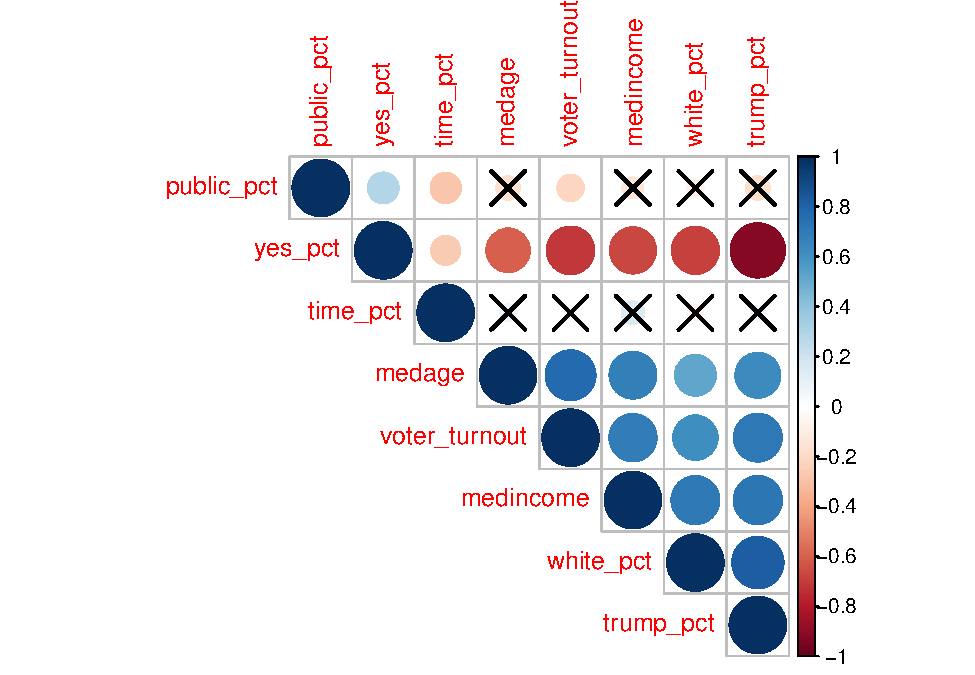
\includegraphics{Zhong_paper_files/figure-latex/create correlation matrix-1.pdf}

\emph{Table 2} lists the summary statistics. Median income is skewed to
the right, with a few tracts demonstrating high income levels. Such a
pattern of inequality is universally observed.

The usage of public transit is low. On average, only one percent of the
population relies on public transportation to go to work. As proved by
later analyses, the distribution is highly skewed, and will be
transformed in some models. \textbf{public\_pct max needs to be fixed}

The variable \emph{current\_plan} is not in \emph{Table 2} because it is
a categorical variable. In sum, 31 tracts do not have access to public
transport within 500 meters, both now and in the short-range. There is
one tract that is categorized as 2, indicating that it has public
transit at present, but not in the short-range proposition. It could be
due to the plan of reducing circuitous routing. Twenty-two tracts do not
enjoy the proximity of public transport now, but will in the
short-range. Lastly, 59 tracts have public transit available both at
present and in the short-range plan. Since a level of this variable
contains only one value (``2''), problems with degrees of freedom will
potentially arise.

A correlation matrix is created from \texttt{corrplot} package to
investigate the correlation between each pair of factors (see
\emph{Figure ???}). Positive correlations are in blue colors, and
negative correlations are in red colors. The magnitude is reflected by
the color intensity and the size of the dot. Non-significant (p
\textgreater{} 0.05) correlations are marked with a cross.
\emph{Current\_plan} is omitted in the matrix because it is categorical.
The dependent variable \emph{yes\_pct} is significantly correlated with
every independent variable. \emph{Medage}, \emph{voter\_turnout},
\emph{medincome}, \emph{white\_pct}, and \emph{trump\_pct} are all
strongly positively correlated with each other, and all of them are
negatively associated with \emph{yes\_pct}. Given the number of strong,
significant correlations among the factors, it is essential to check
collinearity in the regression model.

The major limitation of the data is the unit conversion from precinct to
census tract. Such a method assumes that residents in one precinct have
the same characteristics, and population density is identical. Clearly,
the assumptions cannot be satisfied in a real dataset.

\hypertarget{model-specification}{%
\subsection{Model specification}\label{model-specification}}

Four models are tested in the analysis.

Model 1 adopts linear regression model with all the original variables:

\(yes\_pct_t = \beta_0+\beta_1medincome_t+\beta_2white\_pct_t+\beta_3trump\_pct_t+\beta_4current\_plan_t+\beta_5medage_t+\beta_6public\_pct_t+\beta_7time\_pct_t+\beta_8voter\_turnout_t+\epsilon_t\)

where \(t\) indexes census tract. Since all variables are measured in
the same scope, no fixed effects are tested. The dependent variable is
\emph{yes\_pct}, the proportion of supporters of the referendum in a
tract. Independent variables include \emph{medincome},
\emph{white\_pct}, \emph{trump\_pct}, and \emph{current\_plan}. For more
information about these variables, refer to \emph{Table ???}. I
hypothesize that the effect of \emph{medincome} is ambiguous. As
explained in the Conceptual Model section, people with higher income pay
a larger amount of tax, but the tax takes up a smaller portion of their
earnings compared to those with lower income. \emph{White\_pct} is
hypothesized to have a negative effect on \emph{yes\_pct}, based on the
negative correlation between the two variables. A higher percentage of
Trump supporters is expected to predict a lower percentage of votes for
``yes'' in the referendum, as evidenced by common sense and previous
literature (???). Finally, since tracts that do not have public transit
now and will have it in the short-range benefit the most from the
proposition, I predict that the tracts with this feature will have a
higher level of \emph{yes\_pct} than the others.

\emph{Medage}, \emph{public\_pct}, \emph{time\_pct}, and
\emph{voter\_turnout} add to the model as controls. For example, tracts
with higher voter turnout are hypothesized to have a lower
\emph{yes\_pct}, according to the rule of loss aversion -- people who
believe the referendum incur losses to them are inclined to participate
in the referendum actively and vote against it, but people who like the
proposition are less motivated to vote in nature.

\emph{Medincome}, \emph{public\_pct} and \emph{voter\_turnout} are found
to be positively skewed. Thus, Model 2 uses multiple linear regression
after log or square root transformation on these three variables. Among
them, since many of the values in \emph{public\_pct} are 0, a constant
has to add to the variable before taking log transformation.

\(yes\_pct_t = \beta_0+\beta_1log(medincome_t)+\beta_2white\_pct_t+\beta_3trump\_pct_t+\beta_4current\_plan_t+\beta_5medage_t+\beta_6log(public\_pct_t + 0.01)+\beta_7time\_pct_t+\beta_8\sqrt{voter\_turnout_t}+\epsilon_t\)

\hypertarget{results-discussion}{%
\section{Results \& Discussion}\label{results-discussion}}

\hypertarget{regression-results}{%
\subsection{Regression results}\label{regression-results}}

\begin{table}[!htbp] \centering 
  \caption{Primary regression} 
  \label{Primary} 
\begin{tabular}{@{\extracolsep{5pt}}lc} 
\\[-1.8ex]\hline 
\hline \\[-1.8ex] 
 & \multicolumn{1}{c}{\textit{Dependent variable:}} \\ 
\cline{2-2} 
\\[-1.8ex] & yes\_pct \\ 
\hline \\[-1.8ex] 
 medincome & 0.00000 \\ 
  & (0.00000) \\ 
  & \\ 
 white\_pct & 0.114$^{**}$ \\ 
  & (0.053) \\ 
  & \\ 
 trump\_pct & $-$0.886$^{***}$ \\ 
  & (0.057) \\ 
  & \\ 
 current\_plan2 & 0.019 \\ 
  & (0.044) \\ 
  & \\ 
 current\_plan3 & $-$0.032$^{***}$ \\ 
  & (0.012) \\ 
  & \\ 
 current\_plan4 & 0.016 \\ 
  & (0.012) \\ 
  & \\ 
 medage & 0.003$^{*}$ \\ 
  & (0.001) \\ 
  & \\ 
 public\_pct & 0.817$^{**}$ \\ 
  & (0.338) \\ 
  & \\ 
 time\_pct & $-$0.306$^{***}$ \\ 
  & (0.090) \\ 
  & \\ 
 voter\_turnout & $-$0.326$^{**}$ \\ 
  & (0.126) \\ 
  & \\ 
 Constant & 0.804$^{***}$ \\ 
  & (0.047) \\ 
  & \\ 
\hline \\[-1.8ex] 
Observations & 113 \\ 
R$^{2}$ & 0.917 \\ 
Adjusted R$^{2}$ & 0.909 \\ 
Residual Std. Error & 0.042 (df = 102) \\ 
F Statistic & 113.224$^{***}$ (df = 10; 102) \\ 
\hline 
\hline \\[-1.8ex] 
\textit{Note:}  & \multicolumn{1}{l}{$^{*}$p$<$0.1; $^{**}$p$<$0.05; $^{***}$p$<$0.01} \\ 
\end{tabular} 
\end{table}

\emph{Table ???} provides the results of Model 1. The equation is
statistically significant (F(10, 102) = 113.22, p \textless{} 0.05).
Adjusted \(R^2\) is 0.909, indicating that the independent variables in
this specification explain a large portion of the variance in the
dependent variable. Consistent with the hypothesis, \emph{medincome} is
not a significant predictor of \emph{yes\_pct}. \emph{Trump\_pct}
significantly predicts \emph{yes\_pct} as expected, and results in a
large coefficient: a one percent increase in the proportion of Trump
supporters decreases the percentage of voters in favor of the referendum
by 0.886\%, holding other variables constant.

However, unlike the outcome from the correlation matrix (see
\emph{Figure ???}), \emph{white\_pct} significantly predicts
\emph{yes\_pct} in a positive direction. A higher percentage of the
white population in the tract is associated with higher support of the
proposition when holding other explanatory variables constant.

Another unanticipated result is \emph{current\_plan}. In contrast to
baseline tracts that do not access public transit service both now and
in the short-range (\emph{current\_plan 1}), only \emph{current\_plan 3}
tracts differ from them significantly, in the opposite direction to the
hypothesis. That is to say, tracts planned to be newly added to the
public transit service have a significantly higher rejection of the
proposition than the other tracts. The control variables are all
significant factors. \emph{Medage} and \emph{public\_pct} positively
predict the level of \emph{yes\_pct}, while \emph{time\_pct} and
\emph{voter\_turnout} negatively predict \emph{yes\_pct}.

\begin{table}[!htbp] \centering 
  \caption{Transformed regression} 
  \label{Transformed} 
\begin{tabular}{@{\extracolsep{5pt}}lc} 
\\[-1.8ex]\hline 
\hline \\[-1.8ex] 
 & \multicolumn{1}{c}{\textit{Dependent variable:}} \\ 
\cline{2-2} 
\\[-1.8ex] & yes\_pct \\ 
\hline \\[-1.8ex] 
 log\_medincome & $-$0.008 \\ 
  & (0.022) \\ 
  & \\ 
 white\_pct & 0.117$^{**}$ \\ 
  & (0.051) \\ 
  & \\ 
 trump\_pct & $-$0.857$^{***}$ \\ 
  & (0.059) \\ 
  & \\ 
 current\_plan2 & 0.021 \\ 
  & (0.043) \\ 
  & \\ 
 current\_plan3 & $-$0.033$^{***}$ \\ 
  & (0.012) \\ 
  & \\ 
 current\_plan4 & 0.014 \\ 
  & (0.011) \\ 
  & \\ 
 medage & 0.004$^{**}$ \\ 
  & (0.002) \\ 
  & \\ 
 log\_public\_pct & 0.022$^{***}$ \\ 
  & (0.008) \\ 
  & \\ 
 time\_pct & $-$0.281$^{***}$ \\ 
  & (0.090) \\ 
  & \\ 
 sqrt\_voter\_turnout & $-$0.319$^{***}$ \\ 
  & (0.103) \\ 
  & \\ 
 Constant & 1.032$^{***}$ \\ 
  & (0.219) \\ 
  & \\ 
\hline \\[-1.8ex] 
Observations & 113 \\ 
R$^{2}$ & 0.920 \\ 
Adjusted R$^{2}$ & 0.912 \\ 
Residual Std. Error & 0.041 (df = 102) \\ 
F Statistic & 117.561$^{***}$ (df = 10; 102) \\ 
\hline 
\hline \\[-1.8ex] 
\textit{Note:}  & \multicolumn{1}{l}{$^{*}$p$<$0.1; $^{**}$p$<$0.05; $^{***}$p$<$0.01} \\ 
\end{tabular} 
\end{table}

Model 2 uses multiple linear regression as well, except that the skewed
variables \emph{medincome}, \emph{public\_pct}, and
\emph{voter\_turnout} are transformed. The overall outcome is identical
to Model 1 (see \emph{Table ???}). After log transformation, the effect
of median income is still insignificant.

A series of assumptions are examined. First, linearity and
homoscedasticity assumptions are met, as illustrated by the residual
plots. Next, because several factors correlate with each other (see
\emph{Figure ???}), VIFs are calculated to detect multicollinearity.
Since all of the independent variables exhibit a VIF below 5 in both
models, no collinearity issue is detected. Lastly, there is a potential
fault of using linear regression in this dataset. The value of the
dependent variable \emph{yes\_pct} is restricted to the range of 0 to 1,
because it represents a percentage. On the other hand, the predicted
outcome from linear regression is unbounded. As a result, I calculate
the predicted values from the two models with the actual datasets. The
predicted outcome is close to the actual value of \emph{yes\_pct}, all
between 0 and 1. Then, I continue testing by finding the minimum and
maximum values of each independent variable in the dataset (to see the
actual minimum and maximum values, see \emph{Table ???}), and plug them
into the models accordingly to gain the extreme predicted
\emph{yes\_pct}. The extreme values for Model 1 are 0.09 and 0.96, and
0.11 and 0.95 in Model 2, all within the interval {[}0,1{]}. Therefore,
the range of the dependent variable in these two regression models meets
the assumption.

\hypertarget{discussion}{%
\subsection{Discussion}\label{discussion}}

\hypertarget{mediating-factor}{%
\subsection{Mediating factor}\label{mediating-factor}}

\begin{Shaded}
\begin{Highlighting}[]
\KeywordTok{ggplot}\NormalTok{(final_data, }\KeywordTok{aes}\NormalTok{(}\DataTypeTok{x =}\NormalTok{ white_pct, }\DataTypeTok{y =}\NormalTok{ yes_pct))}\OperatorTok{+}
\StringTok{   }\KeywordTok{geom_point}\NormalTok{()}
\end{Highlighting}
\end{Shaded}

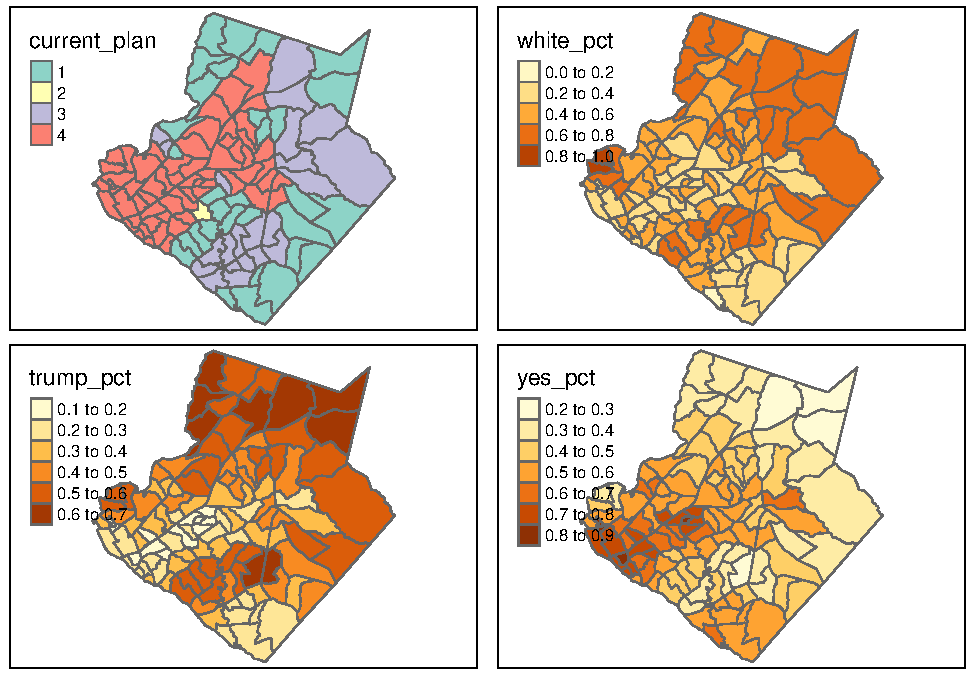
\includegraphics{Zhong_paper_files/figure-latex/unnamed-chunk-2-1.pdf}

\begin{Shaded}
\begin{Highlighting}[]
\KeywordTok{library}\NormalTok{(psych)}
\end{Highlighting}
\end{Shaded}

\begin{verbatim}
## Warning: package 'psych' was built under R version 3.5.3
\end{verbatim}

\begin{verbatim}
## 
## Attaching package: 'psych'
\end{verbatim}

\begin{verbatim}
## The following object is masked from 'package:car':
## 
##     logit
\end{verbatim}

\begin{verbatim}
## The following object is masked from 'package:dlookr':
## 
##     describe
\end{verbatim}

\begin{verbatim}
## The following object is masked from 'package:Hmisc':
## 
##     describe
\end{verbatim}

\begin{verbatim}
## The following objects are masked from 'package:ggplot2':
## 
##     %+%, alpha
\end{verbatim}

\begin{Shaded}
\begin{Highlighting}[]
\KeywordTok{mediate}\NormalTok{(yes_pct }\OperatorTok{~}\StringTok{ }\NormalTok{white_pct }\OperatorTok{+}\StringTok{ }\NormalTok{(trump_pct), }\DataTypeTok{data =}\NormalTok{ final_data, }\DataTypeTok{n.iter =} \DecValTok{10000}\NormalTok{)}
\end{Highlighting}
\end{Shaded}

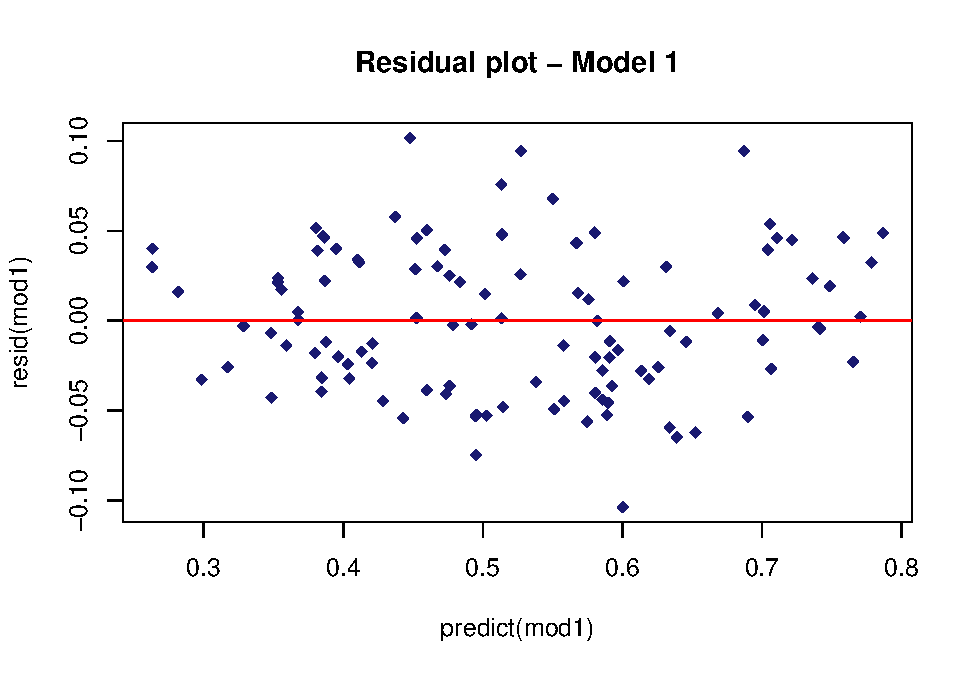
\includegraphics{Zhong_paper_files/figure-latex/unnamed-chunk-3-1.pdf}

\hypertarget{references}{%
\section{References}\label{references}}

\end{document}
